\section{Test Strategy}
\label{sec:test_stra}

The validation has to demonstrate that the openETCS tool chain covers all the functionality. This test strategy will be divided in four sides, the building test, installation test, functional test and performance test:
\begin{itemize}
\item Building testing: The main objective is to check the correct building of the toolchain.
\item Installation test objective: The main objective will be to validate that the OpenETCS platform and the plugins, are correctly installed, and their interoperability is correctly working.
\item Functional test objective: The main objective will be validating that the user’s workflows are correctly created and to provide clear evidence that the platform performs as it should in every possible environment.
\item Performance testing: The main objective is to verify the performance of the tool chain.
\end{itemize}

\section{Test Items}
\label{sec:test_items}
\todo[color=yellow!20, inline]{IT: Brief introduction to the figure. Explanation about how it will grow -according to new feature requests and the
needs of openETCS participants-}


\begin{figure}[htbp]
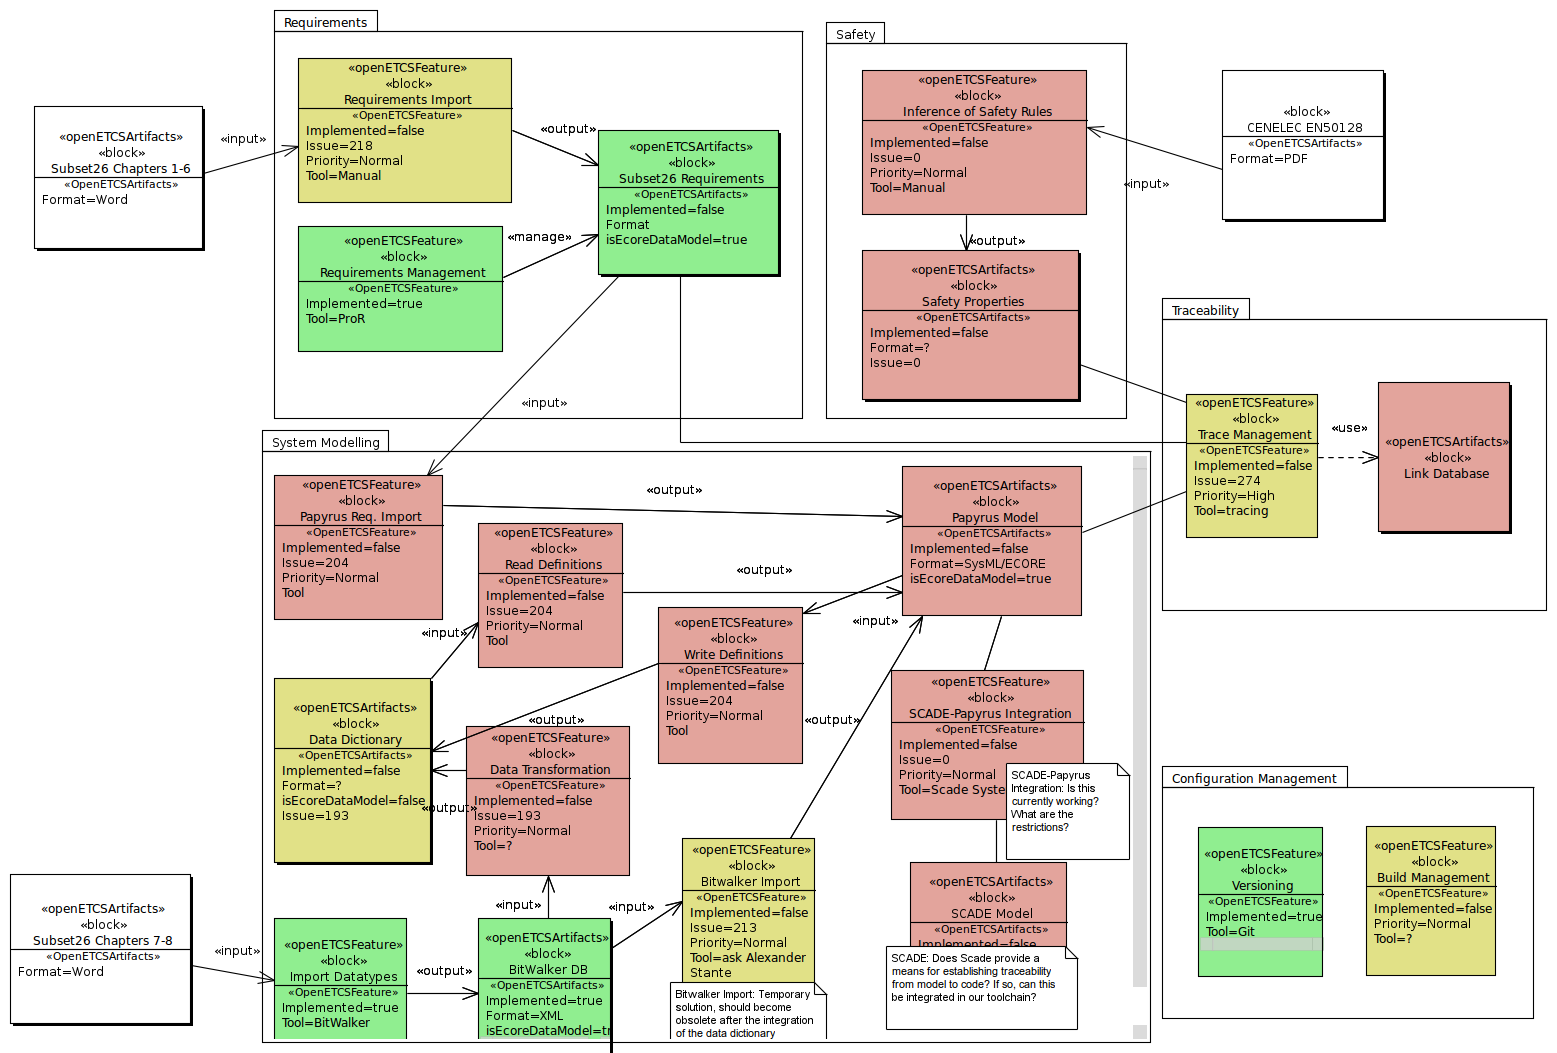
\includegraphics[width=\textwidth]{ToolChainmodel}
\caption{\label{fig:overview} Tool Chain overview (20.02.14) -- \\
  Green Block: Implemented \\
  Yellow Block: Work in Progress \\
  Red Block: Not started \\
  White Block: External Artifacts} 
\end{figure}

The features may be implemented by one or more tools and may also be implemented as plugins.

Currently, openETCS tool chain consists of the following components:
\begin{itemize}
\item Eclipse Kepler
\item Eclipse Modeling Tools
\item Eclipse Papyrus
\item Eclipse RMF
\item Eclipse EGit
\item openETCS documentation
\item openETCS DataDictionary 
\item openETCS tracing
\end{itemize}

The plugins that are going to be part of the first release of the test plan will be:
\begin{itemize}
\item \textbf{Data Dictionary}: This plugin contains the data dictionary plugin which contains data structures, variables, messages, etc. from the ETCS System Requirements Specification (SRS). The plugin registers a UML model, which contains the information from the SRS. After registration, the UML model is available as a UML library.
\item \textbf{Tracing}: The Tracing Features allow the linking of *ProR Requirements* and *SysML Model Elements*. This is realized within the requirements model by using the internal links (SpecRelations) and requirements that act as proxies to the SysML Model element. Note that both, links and proxies, can be extended with additional attributes.
\item \textbf{Documentation}: The documentation plug-in generates Eclipse Help documentation (a hierarchy of HTML files) and PDF documentation from toolchain wiki pages saved as mediawiki.
\end{itemize}

\section{Features to be tested}
\label{sec:features_test}

\begin{center}
\begin{longtable}{|p{2cm}|p{8cm}|}\hline
%\centering
%\begin{tabular}{|p{2cm}|p{8cm}|}\hline
\multicolumn{2}{|c|}{ProR}\\\hline
1 & Check if the RMF documentation is on Eclipse Help\\\hline
2 & Check if is possible to import a ProR requirements model\\\hline
3 & Check if it is possible to import a SysML requirements model\\\hline
4 & Check if it is possible to create a link between ProR and SysML\\\hline
5 & Check if it is possible to add extended attributes to the created links\\\hline
6 & Check how are created the required type of data.\\\hline
7 & Check if it is possible to delete required type of data\\\hline
8 & Check the plugin configuration\\ \hline
9 & ... \\ \hline
\multicolumn{2}{|c|}{Documentation}\\\hline
1 & Check if the documentation is on the eclipse help\\\hline
2 & Check if the links are correct in Eclipse Help\\\hline
3 & Check if the links are correct in the github wiki pages\\\hline
4 & Check if the links are correct in the PDF file\\\hline
5 & ...\\ \hline
\multicolumn{2}{|c|}{Data Dictionary}\\\hline
1 & \\ \hline
%\end{tabular}
\end{longtable}
\end{center}


\section{Item Pass / Fail Criteria}
A test is considered passed when the results obtained are the expected results shown in the Test Case. If any of the expected results are not met, the test is considered failed.

\section{Test Environment}
The environments where is going to be tested the toolchain are based on different operating systems:
\begin{itemize}
\item Windows 64
\item Windows 32
\item Linux 64
\item Linux 32
\item MacOS 64
\item MacOS 32
\end{itemize}

\section{Test Deliverables}
\begin{itemize}
\item Test Specifications
\item Test Results Reports
\item Test Data
\end{itemize}

\section{Schedule}
The plan of tasks related to the activities of the toolchain tests is detailed below:
\begin{table}[H]
\centering
\begin{tabular}{|p{8cm}|p{3cm}|p{3cm}|}\hline
\textbf{Activity} & \textbf{Start Date} & \textbf{End Date}\\\hline
Test Plan Elaboration & & \\\hline
Test Plan Review & & \\\hline
Test Cases Specifications & & \\\hline
Test Cases Review & & \\\hline
Test Cases Execution & & \\\hline
Test Results Report & & \\\hline
\end{tabular}
\end{table}
